% !TEX TS-program = pdflatex
\documentclass[11pt]{article}

% -------------------- Packages --------------------
\usepackage[a4paper,margin=1in]{geometry}
\usepackage{amsmath,amssymb}
\usepackage[T1]{fontenc}
\usepackage{lmodern}
\usepackage{xcolor}
\usepackage{tcolorbox}
\tcbuselibrary{skins,breakable}
\usepackage{enumitem}
\usepackage{hyperref}
\usepackage{tikz}
\usetikzlibrary{arrows.meta,calc,angles,quotes}

\pagestyle{empty}

% -------------------- Dark Theme Colors --------------------
\definecolor{bg}{HTML}{000000}
\definecolor{pairbg}{HTML}{121212}
\definecolor{solbg}{HTML}{0A0A0A}
\definecolor{border}{HTML}{2A2A2A}
\definecolor{text}{HTML}{FFFFFF}
\definecolor{muted}{HTML}{C9CDD3}
\definecolor{gold}{HTML}{FFD700}
\definecolor{green}{HTML}{4ADE80}
\definecolor{cyan}{HTML}{38BDF8}

\pagecolor{bg}
\color{text}

\hypersetup{
  colorlinks=true,
  linkcolor=cyan,
  urlcolor=cyan
}

\setlength{\parindent}{0pt}
\setlength{\parskip}{10pt}

\setlist[itemize]{left=1.4em,itemsep=6pt,topsep=6pt}
\setlist[enumerate]{left=1.6em,itemsep=4pt,topsep=4pt}

% -------------------- tcolorbox Base --------------------
\tcbset{
  enhanced,
  breakable,
  arc=12pt,
  boxrule=0.8pt,
  left=16pt,right=16pt,top=12pt,bottom=12pt
}

\newtcolorbox{QAPair}[1]{%
  colback=pairbg,
  colbacklower=solbg,
  colframe=border,
  coltext=text,
  title=\textcolor{gold}{\bfseries #1},
  fonttitle=\bfseries,
  coltitle=text,
  segmentation style={draw=border, dashed, line width=0.6pt},
}

\newtcolorbox{QuickBox}{%
  colback=pairbg,
  colframe=cyan,
  coltext=text,
  fontupper=\color{text},
  borderline north={4pt}{0pt}{cyan},
  arc=14pt,
  boxrule=0.8pt
}

\newcommand{\Step}[1]{\textcolor{muted}{\textbf{Step #1:}}}

% -------------------- TikZ styles --------------------
\tikzset{
  axes/.style={-Latex, line width=0.8pt, draw=muted},
  grid/.style={draw=border, very thin},
  lineC/.style={line width=1.1pt, draw=cyan},
  lineG/.style={line width=1.1pt, draw=green},
  pt/.style={circle, fill=gold, draw=gold, inner sep=1.6pt},
  lab/.style={text=gold, font=\small},
  labm/.style={text=muted, font=\small}
}

% ============================================================
\begin{document}

\begin{center}
{\LARGE\bfseries \textcolor{gold}{Exercise 8.1 --- Solutions}}\\[-2pt]
\end{center}

\begin{QuickBox}
{\color{cyan}\bfseries Quick formulas (hot topics)}\par\medskip
\begin{itemize}
\item \textbf{Slope / gradient:} $m=\tan\theta$ where $\theta$ is the inclination with the $+x$-axis ($0^\circ \le \theta < 180^\circ$).
\item \textbf{Angle from slope:} $\theta=\tan^{-1}(m)$, but if $m<0$ then take $\theta$ in $(90^\circ,180^\circ)$ (i.e., add $180^\circ$ to the negative acute angle).
\item \textbf{Slope between two points:} If $A(x_1,y_1),\,B(x_2,y_2)$ then $m_{AB}=\dfrac{y_2-y_1}{x_2-x_1}$.
\item \textbf{Parallel lines:} $m_1=m_2$.
\item \textbf{Perpendicular lines:} $m_1m_2=-1$ (non-vertical lines).
\item \textbf{Collinear points:} slopes are equal, e.g. $m_{PQ}=m_{QR}$.
\item \textbf{Parallelogram diagonals:} diagonals bisect each other (midpoints of diagonals are equal).
\end{itemize}
\end{QuickBox}

% ============================================================
% Q1
\begin{QAPair}{Question 1}
\textcolor{gold}{\bfseries Question:} Find the gradient (slope) of a line whose inclination is:
(i) $0^\circ$ \;\; (ii) $30^\circ$ \;\; (iii) $60^\circ$ \;\; (iv) $90^\circ$ \;\;
(v) $120^\circ$ \;\; (vi) $150^\circ$ \;\; (vii) $170^\circ$ \;\; (viii) $45.5^\circ$.
\tcblower
\textcolor{green}{\bfseries Answer:}
\[
\begin{aligned}
\Step{1}\;& m=\tan\theta.\\[2pt]
\Step{2}\;&
\begin{array}{rcl}
(i)\; \theta=0^\circ &\Rightarrow& m=\tan 0^\circ=0\\
(ii)\; \theta=30^\circ &\Rightarrow& m=\tan 30^\circ=\dfrac{1}{\sqrt3}\\
(iii)\; \theta=60^\circ &\Rightarrow& m=\tan 60^\circ=\sqrt3\\
(iv)\; \theta=90^\circ &\Rightarrow& m=\tan 90^\circ\ \text{is undefined (vertical line)}\\
(v)\; \theta=120^\circ &\Rightarrow& m=\tan 120^\circ=-\sqrt3\\
(vi)\; \theta=150^\circ &\Rightarrow& m=\tan 150^\circ=-\dfrac{1}{\sqrt3}\\
(vii)\; \theta=170^\circ &\Rightarrow& m=\tan 170^\circ\approx -0.176\\
(viii)\; \theta=45.5^\circ &\Rightarrow& m=\tan 45.5^\circ\approx 1.018
\end{array}
\end{aligned}
\]

\begin{center}
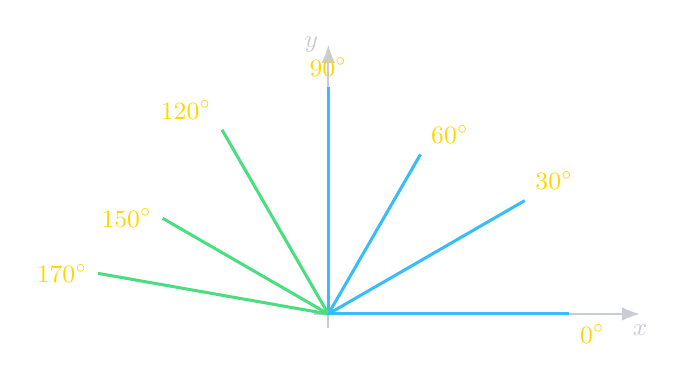
\begin{tikzpicture}[scale=0.9]
  % axes
  \draw[axes] (-0.2,0) -- (4.4,0) node[labm,below] {$x$};
  \draw[axes] (0,-0.2) -- (0,3.8) node[labm,left] {$y$};

  % rays at given angles (representative)
  \draw[lineC] (0,0) -- ({3.2*cos(30)},{3.2*sin(30)}) node[lab,above right] {$30^\circ$};
  \draw[lineC] (0,0) -- ({2.6*cos(60)},{2.6*sin(60)}) node[lab,above right] {$60^\circ$};
  \draw[lineC] (0,0) -- (0,3.2) node[lab,above] {$90^\circ$};

  \draw[lineG] (0,0) -- ({3.0*cos(120)},{3.0*sin(120)}) node[lab,above left] {$120^\circ$};
  \draw[lineG] (0,0) -- ({2.7*cos(150)},{2.7*sin(150)}) node[lab,left] {$150^\circ$};
  \draw[lineG] (0,0) -- ({3.3*cos(170)},{3.3*sin(170)}) node[lab,left] {$170^\circ$};

  \draw[lineC] (0,0) -- (3.4,0) node[lab,below right] {$0^\circ$};
\end{tikzpicture}
\end{center}
\end{QAPair}

% ============================================================
% Q2
\begin{QAPair}{Question 2}
\textcolor{gold}{\bfseries Question:} Find inclination of the line whose slope is:
(i) $0$ \;\; (ii) $0.577$ \;\; (iii) $-1.732$ \;\; (iv) $-0.364$.
\tcblower
\textcolor{green}{\bfseries Answer:}
\[
\begin{aligned}
\Step{1}\;& m=\tan\theta,\quad 0^\circ\le\theta<180^\circ.\\[2pt]
\Step{2}\;&
\begin{array}{rcl}
(i)\; m=0 &\Rightarrow& \theta=0^\circ\\
(ii)\; m=0.577\approx \tan 30^\circ &\Rightarrow& \theta=30^\circ\\
(iii)\; m=-1.732\approx -\sqrt3=\tan 120^\circ &\Rightarrow& \theta=120^\circ\\
(iv)\; m=-0.364\approx \tan 160^\circ &\Rightarrow& \theta=160^\circ
\end{array}
\end{aligned}
\]

\begin{center}
\begin{tikzpicture}[scale=0.9]
  \draw[axes] (-0.2,0) -- (4.4,0) node[labm,below] {$x$};
  \draw[axes] (0,-0.2) -- (0,3.6) node[labm,left] {$y$};
  \draw[lineC] (0,0) -- (3.6,0) node[lab,below right] {$m=0$};
  \draw[lineC] (0,0) -- (3.2,1.85) node[lab,above right] {$m>0$};
  \draw[lineG] (0,0) -- (-3.0,1.1) node[lab,above left] {$m<0\Rightarrow \theta\in(90^\circ,180^\circ)$};
\end{tikzpicture}
\end{center}
\end{QAPair}

% ============================================================
% Q3
\begin{QAPair}{Question 3 (i)}
\textcolor{gold}{\bfseries Question:} Find gradient and inclination of the line joining $A(2,6)$ and $B(5,8)$.
\tcblower
\textcolor{green}{\bfseries Answer:}
\[
\begin{aligned}
\Step{1}\;& m_{AB}=\frac{8-6}{5-2}=\frac{2}{3}.\\
\Step{2}\;& \theta=\tan^{-1}\!\left(\frac{2}{3}\right)\approx 33.69^\circ.
\end{aligned}
\]

\begin{center}
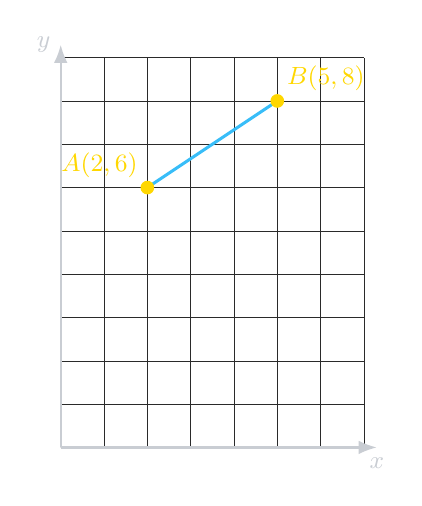
\begin{tikzpicture}[scale=0.55]
  \draw[grid] (0,0) grid (7,9);
  \draw[axes] (0,0) -- (7.3,0) node[labm,below] {$x$};
  \draw[axes] (0,0) -- (0,9.3) node[labm,left] {$y$};

  \coordinate (A) at (2,6);
  \coordinate (B) at (5,8);

  \draw[lineC] (A)--(B);
  \node[pt] at (A) {};
  \node[pt] at (B) {};
  \node[lab,above left] at (A) {$A(2,6)$};
  \node[lab,above right] at (B) {$B(5,8)$};
\end{tikzpicture}
\end{center}
\end{QAPair}

\begin{QAPair}{Question 3 (ii)}
\textcolor{gold}{\bfseries Question:} Find gradient and inclination of the line joining $C(-2,4)$ and $D(1,-3)$.
\tcblower
\textcolor{green}{\bfseries Answer:}
\[
\begin{aligned}
\Step{1}\;& m_{CD}=\frac{-3-4}{1-(-2)}=\frac{-7}{3}.\\
\Step{2}\;& \tan\theta=-\frac{7}{3}\Rightarrow \theta\in(90^\circ,180^\circ).\\
\Step{3}\;& \theta\approx 113.20^\circ.
\end{aligned}
\]

\begin{center}
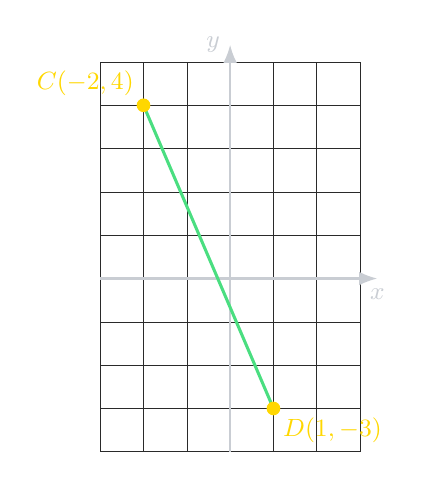
\begin{tikzpicture}[scale=0.55]
  \draw[grid] (-3,-4) grid (3,5);
  \draw[axes] (-3,0) -- (3.4,0) node[labm,below] {$x$};
  \draw[axes] (0,-4) -- (0,5.4) node[labm,left] {$y$};

  \coordinate (C) at (-2,4);
  \coordinate (D) at (1,-3);

  \draw[lineG] (C)--(D);
  \node[pt] at (C) {};
  \node[pt] at (D) {};
  \node[lab,above left] at (C) {$C(-2,4)$};
  \node[lab,below right] at (D) {$D(1,-3)$};
\end{tikzpicture}
\end{center}
\end{QAPair}

\begin{QAPair}{Question 3 (iii)}
\textcolor{gold}{\bfseries Question:} Find gradient and inclination of the line joining $E(5,-2)$ and $F(-2,-3)$.
\tcblower
\textcolor{green}{\bfseries Answer:}
\[
\begin{aligned}
\Step{1}\;& m_{EF}=\frac{-3-(-2)}{-2-5}=\frac{-1}{-7}=\frac{1}{7}.\\
\Step{2}\;& \theta=\tan^{-1}\!\left(\frac{1}{7}\right)\approx 8.13^\circ.
\end{aligned}
\]

\begin{center}
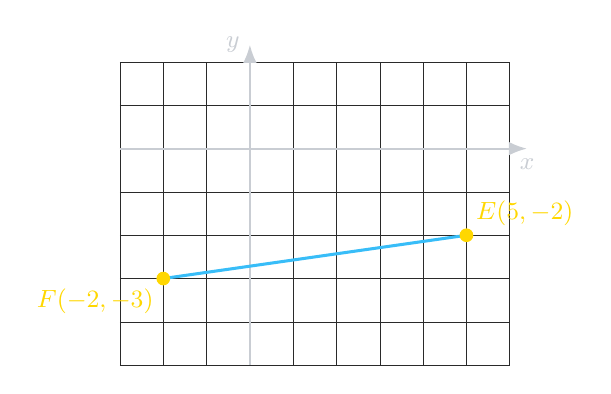
\begin{tikzpicture}[scale=0.55]
  \draw[grid] (-3,-5) grid (6,2);
  \draw[axes] (-3,0) -- (6.4,0) node[labm,below] {$x$};
  \draw[axes] (0,-5) -- (0,2.4) node[labm,left] {$y$};

  \coordinate (E) at (5,-2);
  \coordinate (F) at (-2,-3);

  \draw[lineC] (F)--(E);
  \node[pt] at (E) {};
  \node[pt] at (F) {};
  \node[lab,above right] at (E) {$E(5,-2)$};
  \node[lab,below left] at (F) {$F(-2,-3)$};
\end{tikzpicture}
\end{center}
\end{QAPair}

% ============================================================
% Q4
\begin{QAPair}{Question 4}
\textcolor{gold}{\bfseries Question:} If $A(-2,6)$ and $B(7,-3)$, find the slope of a line:
(i) parallel to $AB$ \;\; (ii) perpendicular to $AB$.
\tcblower
\textcolor{green}{\bfseries Answer:}
\[
\begin{aligned}
\Step{1}\;& m_{AB}=\frac{-3-6}{7-(-2)}=\frac{-9}{9}=-1.\\
\Step{2}\;& \text{Parallel to }AB:\; m=-1.\\
\Step{3}\;& \text{Perpendicular to }AB:\; m\cdot(-1)=-1 \Rightarrow m=1.
\end{aligned}
\]

\begin{center}
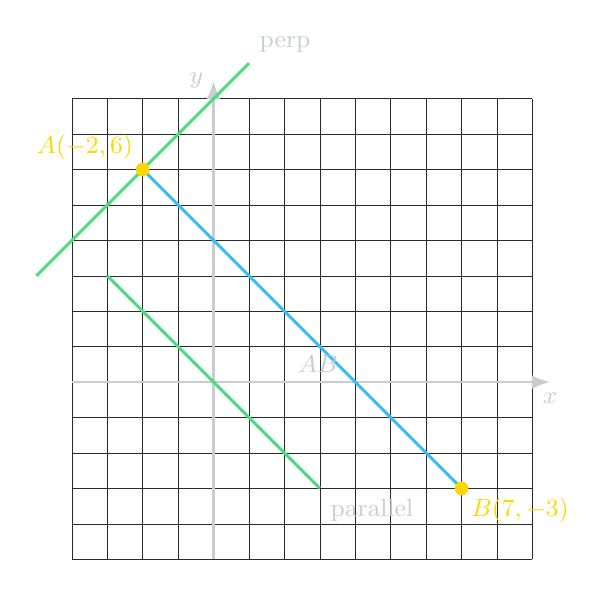
\begin{tikzpicture}[scale=0.45]
  \draw[grid] (-4,-5) grid (9,8);
  \draw[axes] (-4,0) -- (9.5,0) node[labm,below] {$x$};
  \draw[axes] (0,-5) -- (0,8.5) node[labm,left] {$y$};

  \coordinate (A) at (-2,6);
  \coordinate (B) at (7,-3);

  \draw[lineC] (A)--(B) node[pos=0.55,labm,below] {$AB$};
  % a parallel line through origin (slope -1)
  \draw[lineG] (-3,3) -- (3,-3) node[labm,below right] {parallel};
  % a perpendicular line through A (slope 1)
  \draw[lineG] ($(A)+(-3,-3)$) -- ($(A)+(3,3)$) node[labm,above right] {perp};

  \node[pt] at (A) {};
  \node[pt] at (B) {};
  \node[lab,above left] at (A) {$A(-2,6)$};
  \node[lab,below right] at (B) {$B(7,-3)$};
\end{tikzpicture}
\end{center}
\end{QAPair}

% ============================================================
% Q5
\begin{QAPair}{Question 5}
\textcolor{gold}{\bfseries Question:} Find $x$ if the slope of the line passing through $A(3,x)$ and $B(5,8)$ is $4$.
\tcblower
\textcolor{green}{\bfseries Answer:}
\[
\begin{aligned}
\Step{1}\;& m=\frac{8-x}{5-3}=\frac{8-x}{2}.\\
\Step{2}\;& \frac{8-x}{2}=4 \Rightarrow 8-x=8 \Rightarrow x=0.
\end{aligned}
\]

\begin{center}
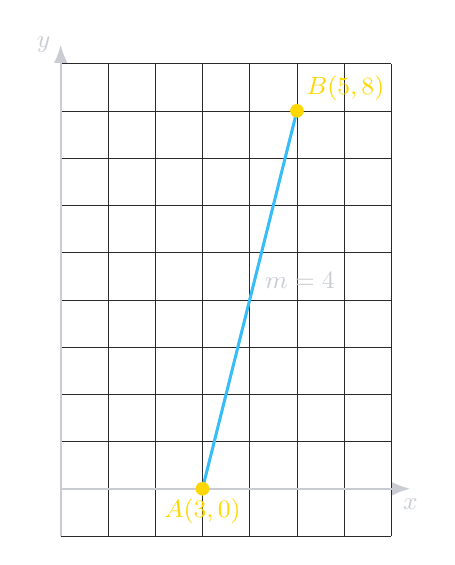
\begin{tikzpicture}[scale=0.6]
  \draw[grid] (0,-1) grid (7,9);
  \draw[axes] (0,0) -- (7.4,0) node[labm,below] {$x$};
  \draw[axes] (0,-1) -- (0,9.4) node[labm,left] {$y$};

  \coordinate (A) at (3,0);
  \coordinate (B) at (5,8);

  \draw[lineC] (A)--(B) node[pos=0.55,labm,right] {$m=4$};
  \node[pt] at (A) {};
  \node[pt] at (B) {};
  \node[lab,below] at (A) {$A(3,0)$};
  \node[lab,above right] at (B) {$B(5,8)$};
\end{tikzpicture}
\end{center}
\end{QAPair}

% ============================================================
% Q6
\begin{QAPair}{Question 6}
\textcolor{gold}{\bfseries Question:} Find $k$ if lines through $A(k,2),B(3,5)$ and $C(5,-1),D(8,7)$ are parallel.
\tcblower
\textcolor{green}{\bfseries Answer:}
\[
\begin{aligned}
\Step{1}\;& m_{AB}=\frac{5-2}{3-k}=\frac{3}{3-k}.\\
\Step{2}\;& m_{CD}=\frac{7-(-1)}{8-5}=\frac{8}{3}.\\
\Step{3}\;& \text{Parallel}\Rightarrow m_{AB}=m_{CD}:\;
\frac{3}{3-k}=\frac{8}{3}.\\
\Step{4}\;& 9=8(3-k)=24-8k \Rightarrow 8k=15 \Rightarrow k=\frac{15}{8}.
\end{aligned}
\]

\begin{center}
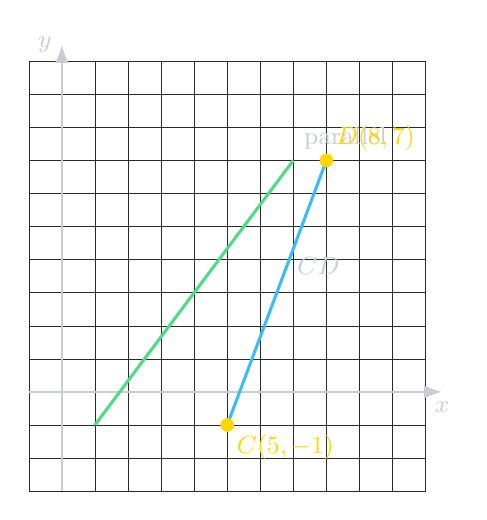
\begin{tikzpicture}[scale=0.42]
  \draw[grid] (-1,-3) grid (11,10);
  \draw[axes] (-1,0) -- (11.5,0) node[labm,below] {$x$};
  \draw[axes] (0,-3) -- (0,10.5) node[labm,left] {$y$};

  \coordinate (C) at (5,-1);
  \coordinate (D) at (8,7);
  \draw[lineC] (C)--(D) node[pos=0.6,labm,right] {$CD$};

  % a parallel guide line
  \draw[lineG] (1,-1) -- (7,7) node[labm,above right] {parallel};

  \node[pt] at (C) {};
  \node[pt] at (D) {};
  \node[lab,below right] at (C) {$C(5,-1)$};
  \node[lab,above right] at (D) {$D(8,7)$};
\end{tikzpicture}
\end{center}
\end{QAPair}

% ============================================================
% Q7
\begin{QAPair}{Question 7}
\textcolor{gold}{\bfseries Question:} Find $k$ if the lines through $P(-1,2),Q(4,7)$ and $R(2,k),S(7,10)$ are perpendicular.
\tcblower
\textcolor{green}{\bfseries Answer:}
\[
\begin{aligned}
\Step{1}\;& m_{PQ}=\frac{7-2}{4-(-1)}=\frac{5}{5}=1.\\
\Step{2}\;& m_{RS}=\frac{10-k}{7-2}=\frac{10-k}{5}.\\
\Step{3}\;& \text{Perpendicular}\Rightarrow m_{PQ}m_{RS}=-1:\\
&\quad 1\cdot\frac{10-k}{5}=-1 \Rightarrow 10-k=-5 \Rightarrow k=15.
\end{aligned}
\]

\begin{center}
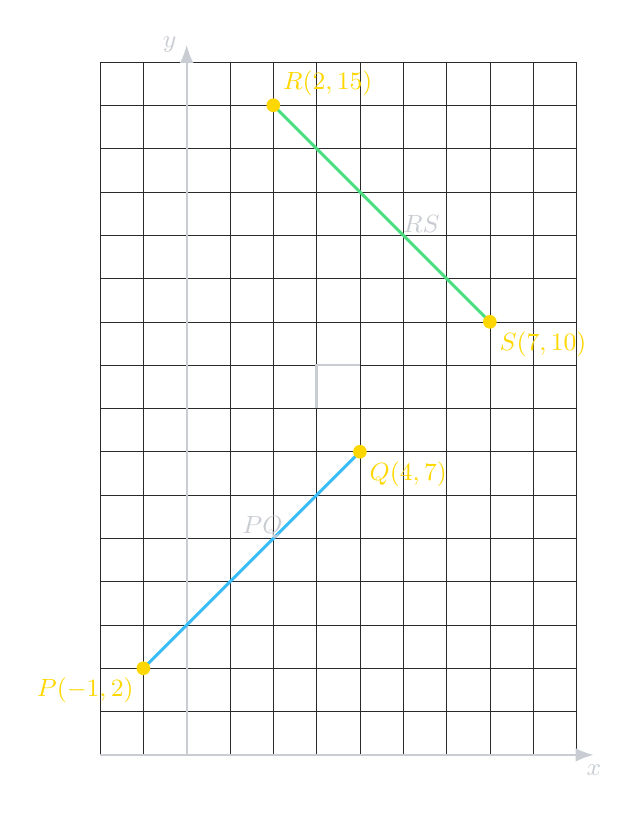
\begin{tikzpicture}[scale=0.55]
  \draw[grid] (-2,0) grid (9,16);
  \draw[axes] (-2,0) -- (9.4,0) node[labm,below] {$x$};
  \draw[axes] (0,0) -- (0,16.4) node[labm,left] {$y$};

  \coordinate (P) at (-1,2);
  \coordinate (Q) at (4,7);

  \draw[lineC] (P)--(Q) node[pos=0.55,labm,above] {$PQ$};

  % perpendicular line drawn through (2,15) to meet the idea of k=15
  \coordinate (R) at (2,15);
  \coordinate (S) at (7,10);
  \draw[lineG] (R)--(S) node[pos=0.55,labm,right] {$RS$};

  \node[pt] at (P) {}; \node[pt] at (Q) {};
  \node[pt] at (R) {}; \node[pt] at (S) {};
  \node[lab,below left] at (P) {$P(-1,2)$};
  \node[lab,below right] at (Q) {$Q(4,7)$};
  \node[lab,above right] at (R) {$R(2,15)$};
  \node[lab,below right] at (S) {$S(7,10)$};

  % right-angle marker near intersection (approx visual)
  \draw[muted, line width=0.8pt] (3,8) -- (3,9) -- (4,9);
\end{tikzpicture}
\end{center}
\end{QAPair}
% ============================================================
% Q8
\begin{QAPair}{Question 8}
\textcolor{gold}{\bfseries Question:} Using slopes, prove that points $X(0,-3)$, $Y(4,7)$ and $Z(6,12)$ are collinear.
\tcblower
\textcolor{green}{\bfseries Answer:}
\[
\begin{aligned}
\Step{1}\;& m_{XY}=\frac{7-(-3)}{4-0}=\frac{10}{4}=\frac{5}{2}.\\
\Step{2}\;& m_{YZ}=\frac{12-7}{6-4}=\frac{5}{2}.\\
\Step{3}\;& m_{XY}=m_{YZ}\ \Rightarrow\ X,Y,Z \text{ lie on the same straight line (collinear).}
\end{aligned}
\]
(Also, $m_{XZ}=\dfrac{12-(-3)}{6-0}=\dfrac{15}{6}=\dfrac{5}{2}$, consistent.)

\textcolor{muted}{\bfseries Sketch:}\par
\begin{center}
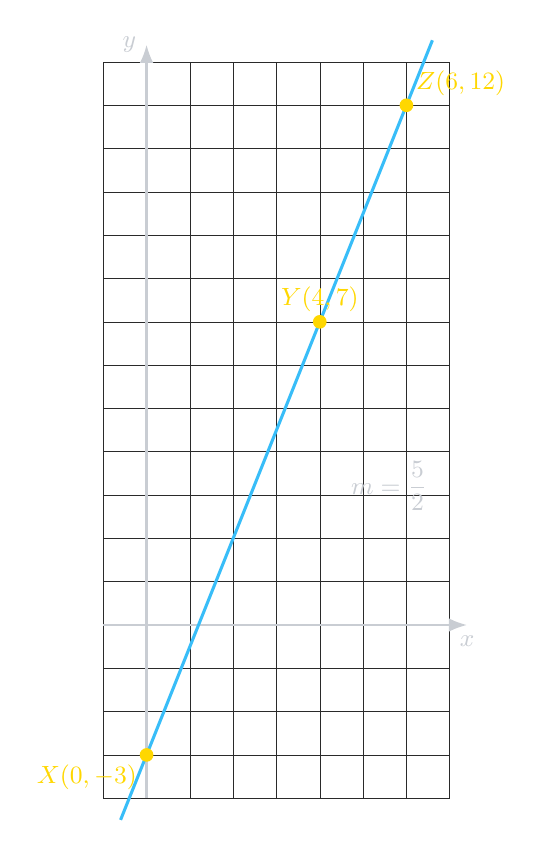
\begin{tikzpicture}[scale=0.55]
  \draw[grid] (-1,-4) grid (7,13);
  \draw[axes] (-1,0) -- (7.4,0) node[labm,below] {$x$};
  \draw[axes] (0,-4) -- (0,13.4) node[labm,left] {$y$};

  \coordinate (X) at (0,-3);
  \coordinate (Y) at (4,7);
  \coordinate (Z) at (6,12);

  % the line through X and Z
  \draw[lineC] ($(X)+(-0.6,-1.5)$) -- ($(Z)+(0.6,1.5)$);

  \node[pt] at (X) {};
  \node[pt] at (Y) {};
  \node[pt] at (Z) {};

  \node[lab,below left] at (X) {$X(0,-3)$};
  \node[lab,above] at (Y) {$Y(4,7)$};
  \node[lab,above right] at (Z) {$Z(6,12)$};

  \node[labm] at (5.6,3.2) {$m=\dfrac{5}{2}$};
\end{tikzpicture}
\end{center}
\end{QAPair}

% ============================================================
% Q9
\begin{QAPair}{Question 9}
\textcolor{gold}{\bfseries Question:} Find $y$ if points $P(4,y)$, $Q(5,2)$ and $R(6,2y+1)$ are collinear.
\tcblower
\textcolor{green}{\bfseries Answer:}
\[
\begin{aligned}
\Step{1}\;& \text{Collinear}\Rightarrow m_{PQ}=m_{QR}.\\
\Step{2}\;& m_{PQ}=\frac{2-y}{5-4}=2-y.\\
\Step{3}\;& m_{QR}=\frac{(2y+1)-2}{6-5}=2y-1.\\
\Step{4}\;& 2-y=2y-1 \Rightarrow 3y=3 \Rightarrow y=1.
\end{aligned}
\]

\begin{center}
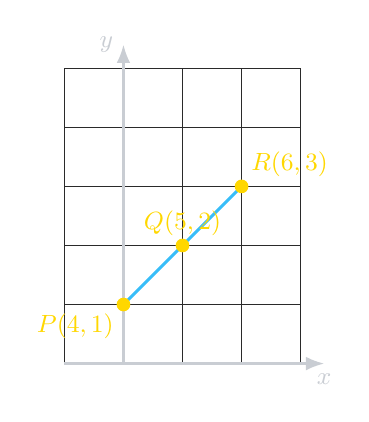
\begin{tikzpicture}[scale=0.75]
  \draw[grid] (3,0) grid (7,5);
  \draw[axes] (3,0) -- (7.4,0) node[labm,below] {$x$};
  \draw[axes] (4,0) -- (4,5.4) node[labm,left] {$y$};

  \coordinate (P) at (4,1);
  \coordinate (Q) at (5,2);
  \coordinate (R) at (6,3);

  \draw[lineC] (P)--(R);
  \node[pt] at (P) {}; \node[pt] at (Q) {}; \node[pt] at (R) {};
  \node[lab,below left] at (P) {$P(4,1)$};
  \node[lab,above] at (Q) {$Q(5,2)$};
  \node[lab,above right] at (R) {$R(6,3)$};
\end{tikzpicture}
\end{center}
\end{QAPair}

% ============================================================
% Q10
\begin{QAPair}{Question 10}
\textcolor{gold}{\bfseries Question:} Prove by using slopes that $A(3,-1)$, $B(-5,-5)$ and $C(1,3)$ are vertices of a right-angled triangle.
\tcblower
\textcolor{green}{\bfseries Answer:}
\[
\begin{aligned}
\Step{1}\;& m_{AB}=\frac{-5-(-1)}{-5-3}=\frac{-4}{-8}=\frac12.\\
\Step{2}\;& m_{AC}=\frac{3-(-1)}{1-3}=\frac{4}{-2}=-2.\\
\Step{3}\;& m_{AB}\cdot m_{AC}=\frac12\cdot(-2)=-1
\;\Rightarrow\; AB\perp AC.\\
\Step{4}\;& \therefore\ \triangle ABC \text{ is right-angled at }A.
\end{aligned}
\]

\begin{center}
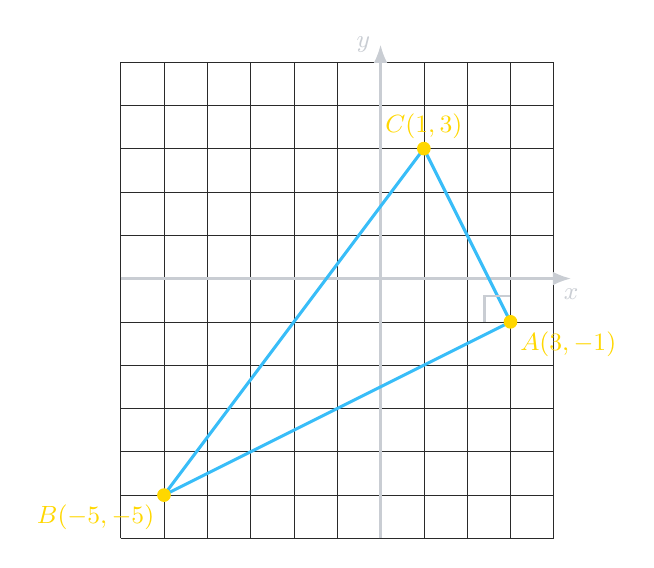
\begin{tikzpicture}[scale=0.55]
  \draw[grid] (-6,-6) grid (4,5);
  \draw[axes] (-6,0) -- (4.4,0) node[labm,below] {$x$};
  \draw[axes] (0,-6) -- (0,5.4) node[labm,left] {$y$};

  \coordinate (A) at (3,-1);
  \coordinate (B) at (-5,-5);
  \coordinate (C) at (1,3);

  \draw[lineC] (A)--(B)--(C)--cycle;
  \node[pt] at (A) {}; \node[pt] at (B) {}; \node[pt] at (C) {};
  \node[lab,below right] at (A) {$A(3,-1)$};
  \node[lab,below left] at (B) {$B(-5,-5)$};
  \node[lab,above] at (C) {$C(1,3)$};

  % right angle marker at A (visual)
  \draw[muted, line width=0.8pt] ($(A)+(-0.6,0)$) -- ($(A)+(-0.6,0.6)$) -- ($(A)+(0,0.6)$);
\end{tikzpicture}
\end{center}
\end{QAPair}

% ============================================================
% Q11
\begin{QAPair}{Question 11}
\textcolor{gold}{\bfseries Question:} Using slope, prove that $A(-2,1)$, $B(6,3)$, $C(10,5)$ and $D(2,3)$ are vertices of a parallelogram.
\tcblower
\textcolor{green}{\bfseries Answer:}
\[
\begin{aligned}
\Step{1}\;& m_{AB}=\frac{3-1}{6-(-2)}=\frac{2}{8}=\frac14.\\
\Step{2}\;& m_{CD}=\frac{3-5}{2-10}=\frac{-2}{-8}=\frac14
\;\Rightarrow\; AB\parallel CD.\\
\Step{3}\;& m_{BC}=\frac{5-3}{10-6}=\frac{2}{4}=\frac12.\\
\Step{4}\;& m_{AD}=\frac{3-1}{2-(-2)}=\frac{2}{4}=\frac12
\;\Rightarrow\; BC\parallel AD.\\
\Step{5}\;& \therefore\ ABCD\ \text{is a parallelogram.}
\end{aligned}
\]

\begin{center}
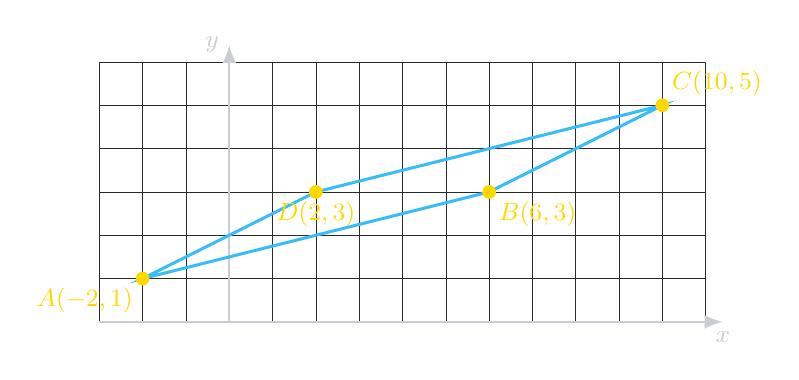
\begin{tikzpicture}[scale=0.55]
  \draw[grid] (-3,0) grid (11,6);
  \draw[axes] (-3,0) -- (11.4,0) node[labm,below] {$x$};
  \draw[axes] (0,0) -- (0,6.4) node[labm,left] {$y$};

  \coordinate (A) at (-2,1);
  \coordinate (B) at (6,3);
  \coordinate (C) at (10,5);
  \coordinate (D) at (2,3);

  \draw[lineC] (A)--(B)--(C)--(D)--cycle;

  \node[pt] at (A) {}; \node[pt] at (B) {}; \node[pt] at (C) {}; \node[pt] at (D) {};
  \node[lab,below left] at (A) {$A(-2,1)$};
  \node[lab,below right] at (B) {$B(6,3)$};
  \node[lab,above right] at (C) {$C(10,5)$};
  \node[lab,below] at (D) {$D(2,3)$};
\end{tikzpicture}
\end{center}
\end{QAPair}

% ============================================================
% Q12
\begin{QAPair}{Question 12}
\textcolor{gold}{\bfseries Question:} $P(x,y)$, $Q(-2,2)$, $R(1,4)$ and $S(10,1)$ are vertices of a parallelogram. Find $P(x,y)$.
\tcblower
\textcolor{green}{\bfseries Answer:}
\[
\begin{aligned}
\Step{1}\;& \text{In parallelogram }PQRS,\ \text{diagonals }PR \text{ and }QS\ \text{bisect each other.}\\
\Step{2}\;& \text{Midpoint of }QS=\left(\frac{-2+10}{2},\frac{2+1}{2}\right)=(4,\tfrac{3}{2}).\\
\Step{3}\;& \text{Midpoint of }PR=\left(\frac{x+1}{2},\frac{y+4}{2}\right).\\
\Step{4}\;& \left(\frac{x+1}{2},\frac{y+4}{2}\right)=(4,\tfrac{3}{2})
\Rightarrow x=7,\ y=-1.\\
\Step{5}\;& \boxed{P(7,-1)}.
\end{aligned}
\]

\begin{center}
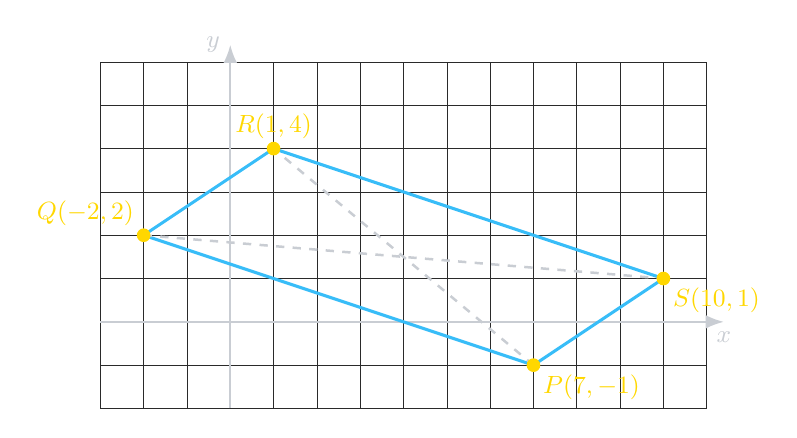
\begin{tikzpicture}[scale=0.55]
  \draw[grid] (-3,-2) grid (11,6);
  \draw[axes] (-3,0) -- (11.4,0) node[labm,below] {$x$};
  \draw[axes] (0,-2) -- (0,6.4) node[labm,left] {$y$};

  \coordinate (Q) at (-2,2);
  \coordinate (R) at (1,4);
  \coordinate (S) at (10,1);
  \coordinate (P) at (7,-1);

  \draw[lineC] (P)--(Q)--(R)--(S)--cycle;

  % diagonals
  \draw[muted, dashed, line width=0.9pt] (P)--(R);
  \draw[muted, dashed, line width=0.9pt] (Q)--(S);

  \node[pt] at (P) {}; \node[pt] at (Q) {}; \node[pt] at (R) {}; \node[pt] at (S) {};
  \node[lab,below right] at (P) {$P(7,-1)$};
  \node[lab,above left] at (Q) {$Q(-2,2)$};
  \node[lab,above] at (R) {$R(1,4)$};
  \node[lab,below right] at (S) {$S(10,1)$};
\end{tikzpicture}
\end{center}
\end{QAPair}

% ============================================================
% Q13
\begin{QAPair}{Question 13}
\textcolor{gold}{\bfseries Question:} Three vertices of a rhombus are $A(2,-1)$, $B(3,4)$ and $C(-2,3)$. Find the fourth vertex.
\tcblower
\textcolor{green}{\bfseries Answer:}
\[
\begin{aligned}
\Step{1}\;& AB=\sqrt{(3-2)^2+(4-(-1))^2}=\sqrt{1+25}=\sqrt{26}.\\
\Step{2}\;& BC=\sqrt{(-2-3)^2+(3-4)^2}=\sqrt{25+1}=\sqrt{26}.\\
\Step{3}\;& AB=BC \Rightarrow A,B,C \text{ can be consecutive vertices.}\\
\Step{4}\;& \text{For parallelogram/rhombus }ABCD,\ D=A+C-B.\\
\Step{5}\;& D=(2,-1)+(-2,3)-(3,4)=(-3,-2).\\
\Step{6}\;& \boxed{D(-3,-2)}.
\end{aligned}
\]

\begin{center}
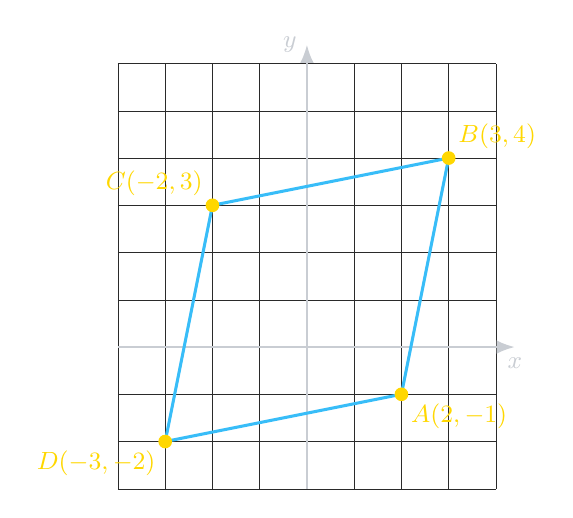
\begin{tikzpicture}[scale=0.6]
  \draw[grid] (-4,-3) grid (4,6);
  \draw[axes] (-4,0) -- (4.4,0) node[labm,below] {$x$};
  \draw[axes] (0,-3) -- (0,6.4) node[labm,left] {$y$};

  \coordinate (A) at (2,-1);
  \coordinate (B) at (3,4);
  \coordinate (C) at (-2,3);
  \coordinate (D) at (-3,-2);

  \draw[lineC] (A)--(B)--(C)--(D)--cycle;

  \node[pt] at (A) {}; \node[pt] at (B) {}; \node[pt] at (C) {}; \node[pt] at (D) {};
  \node[lab,below right] at (A) {$A(2,-1)$};
  \node[lab,above right] at (B) {$B(3,4)$};
  \node[lab,above left] at (C) {$C(-2,3)$};
  \node[lab,below left] at (D) {$D(-3,-2)$};
\end{tikzpicture}
\end{center}
\end{QAPair}

% ============================================================
% Q14
\begin{QAPair}{Question 14}
\textcolor{gold}{\bfseries Question:} If $(5,0)$, $(0,5)$ and $(8,8)$ are vertices of a triangle, find:
(i) slopes of sides \;\; (ii) slopes of medians \;\; (iii) slopes of altitudes.
\tcblower
\textcolor{green}{\bfseries Answer:}
Let $A(5,0)$, $B(0,5)$, $C(8,8)$.

\[
\begin{aligned}
\text{\textcolor{gold}{(i) Slopes of sides}}:\quad
\Step{1}\;& m_{AB}=\frac{5-0}{0-5}=-1.\\
\Step{2}\;& m_{BC}=\frac{8-5}{8-0}=\frac{3}{8}.\\
\Step{3}\;& m_{CA}=\frac{0-8}{5-8}=\frac{8}{3}.\\[6pt]
\text{\textcolor{gold}{(ii) Slopes of medians}}:\quad
\Step{4}\;& M_{BC}\!=\!\left(\frac{0+8}{2},\frac{5+8}{2}\right)=\left(4,\frac{13}{2}\right).\\
& m_{A\!M_{BC}}=\frac{\frac{13}{2}-0}{4-5}=-\frac{13}{2}.\\
\Step{5}\;& M_{CA}\!=\!\left(\frac{8+5}{2},\frac{8+0}{2}\right)=\left(\frac{13}{2},4\right).\\
& m_{B\!M_{CA}}=\frac{4-5}{\frac{13}{2}-0}=-\frac{2}{13}.\\
\Step{6}\;& M_{AB}\!=\!\left(\frac{5+0}{2},\frac{0+5}{2}\right)=\left(\frac{5}{2},\frac{5}{2}\right).\\
& m_{C\!M_{AB}}=\frac{\frac{5}{2}-8}{\frac{5}{2}-8}=1.\\[6pt]
\text{\textcolor{gold}{(iii) Slopes of altitudes}}:\quad
\Step{7}\;& \text{Altitude from }A\perp BC:\ m=-\frac{1}{m_{BC}}=-\frac{8}{3}.\\
\Step{8}\;& \text{Altitude from }B\perp CA:\ m=-\frac{1}{m_{CA}}=-\frac{3}{8}.\\
\Step{9}\;& \text{Altitude from }C\perp AB:\ m=-\frac{1}{m_{AB}}=1.
\end{aligned}
\]

\begin{center}
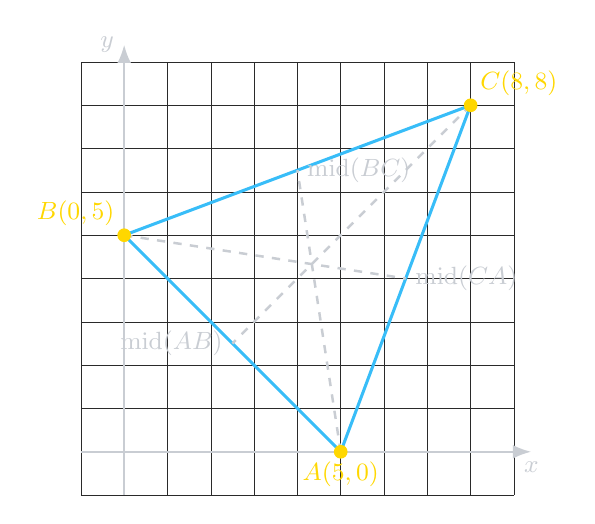
\begin{tikzpicture}[scale=0.55]
  \draw[grid] (-1,-1) grid (9,9);
  \draw[axes] (-1,0) -- (9.4,0) node[labm,below] {$x$};
  \draw[axes] (0,-1) -- (0,9.4) node[labm,left] {$y$};

  \coordinate (A) at (5,0);
  \coordinate (B) at (0,5);
  \coordinate (C) at (8,8);

  \draw[lineC] (A)--(B)--(C)--cycle;

  % Medians (dashed)
  \coordinate (Mbc) at (4,6.5);
  \coordinate (Mca) at (6.5,4);
  \coordinate (Mab) at (2.5,2.5);
  \draw[muted, dashed, line width=0.9pt] (A)--(Mbc);
  \draw[muted, dashed, line width=0.9pt] (B)--(Mca);
  \draw[muted, dashed, line width=0.9pt] (C)--(Mab);

  \node[pt] at (A) {}; \node[pt] at (B) {}; \node[pt] at (C) {};
  \node[lab,below] at (A) {$A(5,0)$};
  \node[lab,above left] at (B) {$B(0,5)$};
  \node[lab,above right] at (C) {$C(8,8)$};

  \node[labm, right] at (Mbc) {mid$(BC)$};
  \node[labm, right] at (Mca) {mid$(CA)$};
  \node[labm, left] at (Mab) {mid$(AB)$};
\end{tikzpicture}
\end{center}
\end{QAPair}

\end{document}
